\documentclass[a4paper]{article}

%% Language and font encodings
\usepackage[english]{babel}
\usepackage[utf8x]{inputenc}
\usepackage[T1]{fontenc}

%% Sets page size and margins
\usepackage[a4paper,top=3cm,bottom=2cm,left=3cm,right=3cm,marginparwidth=1.75cm]{geometry}

%% Useful packages
\usepackage{amsmath}
\usepackage{amssymb}
\usepackage{enumitem}
\usepackage{graphicx}
\usepackage{float}
\usepackage[colorinlistoftodos]{todonotes}
% \usepackage[colorlinks=true, allcolors=blue]{hyperref}
\usepackage{xcolor}
\usepackage{url}

\title{Homework 6\\
	601.482/682 Deep Learning\\
	Fall 2023}
\date{Oct 18, 2023}
\begin{document}
	\maketitle

	\begin{center}
		\textbf{Due 11:59pm on Nov 8, 2023}
	\end{center}
	\begin{center}\textbf{Please submit 1) a single zip file containing your Jupyter Notebook and PDF of your Jupyter Notebook to ``Homework 6 - Notebook'' and 2) your written report (LaTeX generated PDF) to ``Homework 6 - Report'' on Gradescope (Entry Code: BBVDNN)}
	\end{center}

	\noindent \emph{Important:} You must program this homework using the PyTorch framework. We highly recommend using Google Colaboratory.\\

	\noindent \emph{Important:} If you don't have local GPU access, you should port the provided Python scripts to Colaboratory and enable GPU in that environment (under Edit->Notebook Settings). Training should converge in less than 30 min. If your model does not make significant updates in that time, you should re-examine your code. Either way, this is a reminder to start the assignment early.

	\begin{enumerate}
		% Problem 1
		\item \textit{Unsupervised Pre-training}. In this problem, you will attempt the 2017 Endoscopic Instrument Challenge.\footnote{\url{https://endovissub2017-roboticinstrumentsegmentation.grand-challenge.org}} You are given a pre-processed dataset consisting of endoscopic frame images (\emph{not} in sequential order). The goal is to train a network which takes each RGB frame as an input and predicts a pixel-wise segmentation mask that labels the target instrument type and background tissue. Additionally, we introduce an unsupervised pre-training method and compare the performance of training on a small labeled dataset with/without pre-training. This is relevant for real-life medical image problems, where there is usually a shortage of data labels. 
		
		\textbf{Data Folder} 
		We have provided a well-structured dataset. It consists of `/segmentation' and `/colorization'. In each sub-folder, there are `/train' and `/validation' for training purposes. 
		
		The \textbf{main goals} of the homework are as follows. Concrete TODOs are enumerated on the next page.
		
		\begin{itemize}
			\item \textit{Complete the Network structure for segmentation task (a-c)}. The network structure we provide is a simplified U-Net, which is a very popular framework in medical image segmentation task.  Read and understand the code in \texttt{unet.py}, the implementation is missing the last layer and the last activation function. Next, fill in the missing components for 1(a). For the segmentation task, train ONLY with the frames in `/segmentation/train' and validate and test with the frames in `/segmentation/validation' and `/segmentation/test' respectively. The original input image is a $256 \times 320 \times 3$ RGB image. The ground truth label is a grey-scale image that has the same dimension, where different gray values indicate the instrument type or background tissue. 
			
			
			\item \textit{Pre-training by self-supervised colorization (d)}.  Image colorization training\footnote{Larsson, G., Maire, M., \& Shakhnarovich, G. (2017). Colorization as a proxy task for visual understanding. In Proceedings of the IEEE Conference on Computer Vision and Pattern Recognition (pp. 6874-6883).} is a common way of self-supervised learning.\footnote{Jing, L., \& Tian, Y. (2020). Self-supervised visual feature learning with deep neural networks: A survey. IEEE Transactions on Pattern Analysis and Machine Intelligence.} The idea is to take grey-scale images as an input and predict colorized images, similar to filling in colors in a draft painting. You must use the \textbf{same} U-Net structure as above to train a model for this colorization task. Then use the pretrained weights as initialization for the segmentation task.
			
			For the colorization task, you need to train on `/colorization/train\_cor' and validate on `/colorization/validation\_cor'. You are given \texttt{mapping.json} that contains the label of each grey level. We have also provided grey-scale image for each input in each subfolder of `/colorization' for your colorization task input.
			

		\end{itemize}
		Now that you know the broad goals and data sets, please complete the following TODOs.
		\begin{enumerate}
			\item Train a segmentation network using the frames in the `/segmentation/train' folder. Please complete the DICE score function to evaluate your model, and write from scratch a DICE loss function as your network loss\footnote{Read more about the DICE score: \url{https://medium.com/datadriveninvestor/deep-learning-in-medical-imaging-3c1008431aaf}}. (\textit{Hint: You need to convert the grey-scale label mask to one-hot encoding of the label and then calculate the DICE score for each label}). Please train the network until convergence (should take around 30 min) using the default provided hyperparameters and provide a figure of training loss and validation loss w.r.t. epochs (in a single figure). Please report your performance (DICE score) on the test dataset, you should expect a DICE score > 0.5. (\textit{Hint: Using BatchNorm might help you achieve better performance.})
			
			\noindent \textbf{Answer for 1(a):} \\
			Figure ~\ref{fig:1a}  is the train loss and validation loss w.r.t. epochs. 
			
			\begin{figure}[h!]
				\centering
				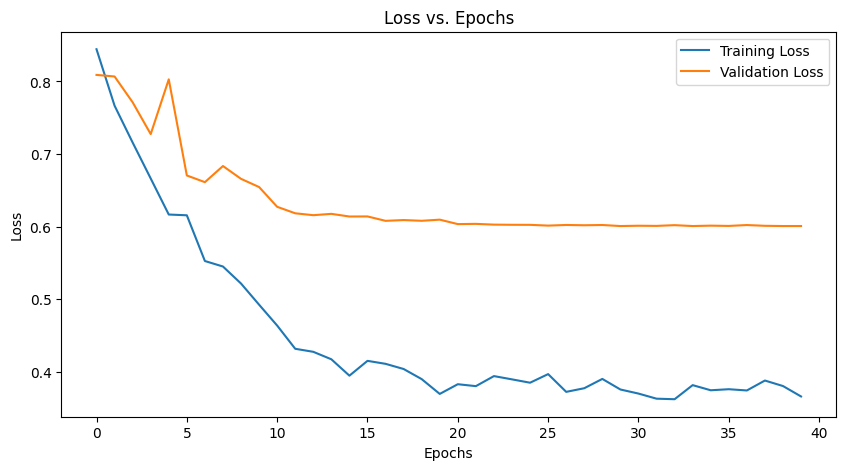
\includegraphics[width=\linewidth]{/Users/zhangxiangyu/JHU/Fall 2023/deep learning/hw6/fig/1a.png}
				\caption{Validation and train loss w.r.t. epochs}
				\label{fig:1a}
			\end{figure}

			The dice score on the test dataset is $0.55$, which can be shown in Figure ~\ref{fig:1a_dice}.
			\begin{figure}[h!]
				\centering
				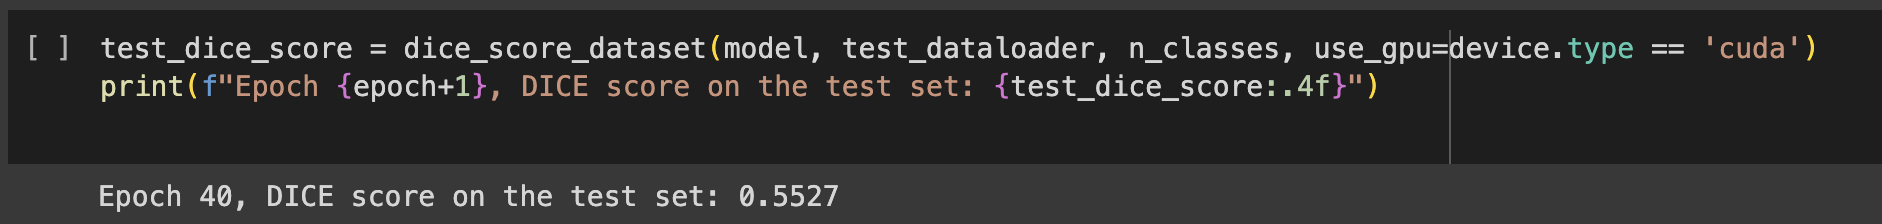
\includegraphics[width= 0.9\textwidth]{/Users/zhangxiangyu/JHU/Fall 2023/deep learning/hw6/fig/1a_dice.png}
				\caption{Dice score on the test dataset}
				\label{fig:1a_dice}
			\end{figure}


			\item Introduce meaningful data augmentation (e.g. vertical and horizontal flips) and train the network until convergence using the same hyperparameters as (a). Please plot the training loss and validation loss on a single figure again and report test dataset performance, you should expect a DICE score > 0.6.
			
			\noindent \textbf{Answer for 1(b):} \\

			I applied random horizontal flip and random rotation for data augmentation. The corresponding train and validation loss can be found in Figure ~\ref{fig:1b}. The dice score on the test dataset is $0.4572$, which can be shown in Figure ~\ref{fig:1b_dice}.
			

			\textbf{Result analysis:} 
			From the result, we can see that the data augmentation decrease the performance of the model. The dice score on the test dataset is decreased from $0.5527$ to $0.4572$. The possible reason is that the model may not have enough capacity to learn the augmented data. For our dataset, we only have 300 images for training, which is not enough for a complex model. Also, U-Net relies on local features and context to make predictions. If the augmentations distort the images too much (e.g., extreme rotations, flips, or color changes that do not occur naturally), the network might fail to learn the correct features.

			\begin{figure}[H]
				\centering
				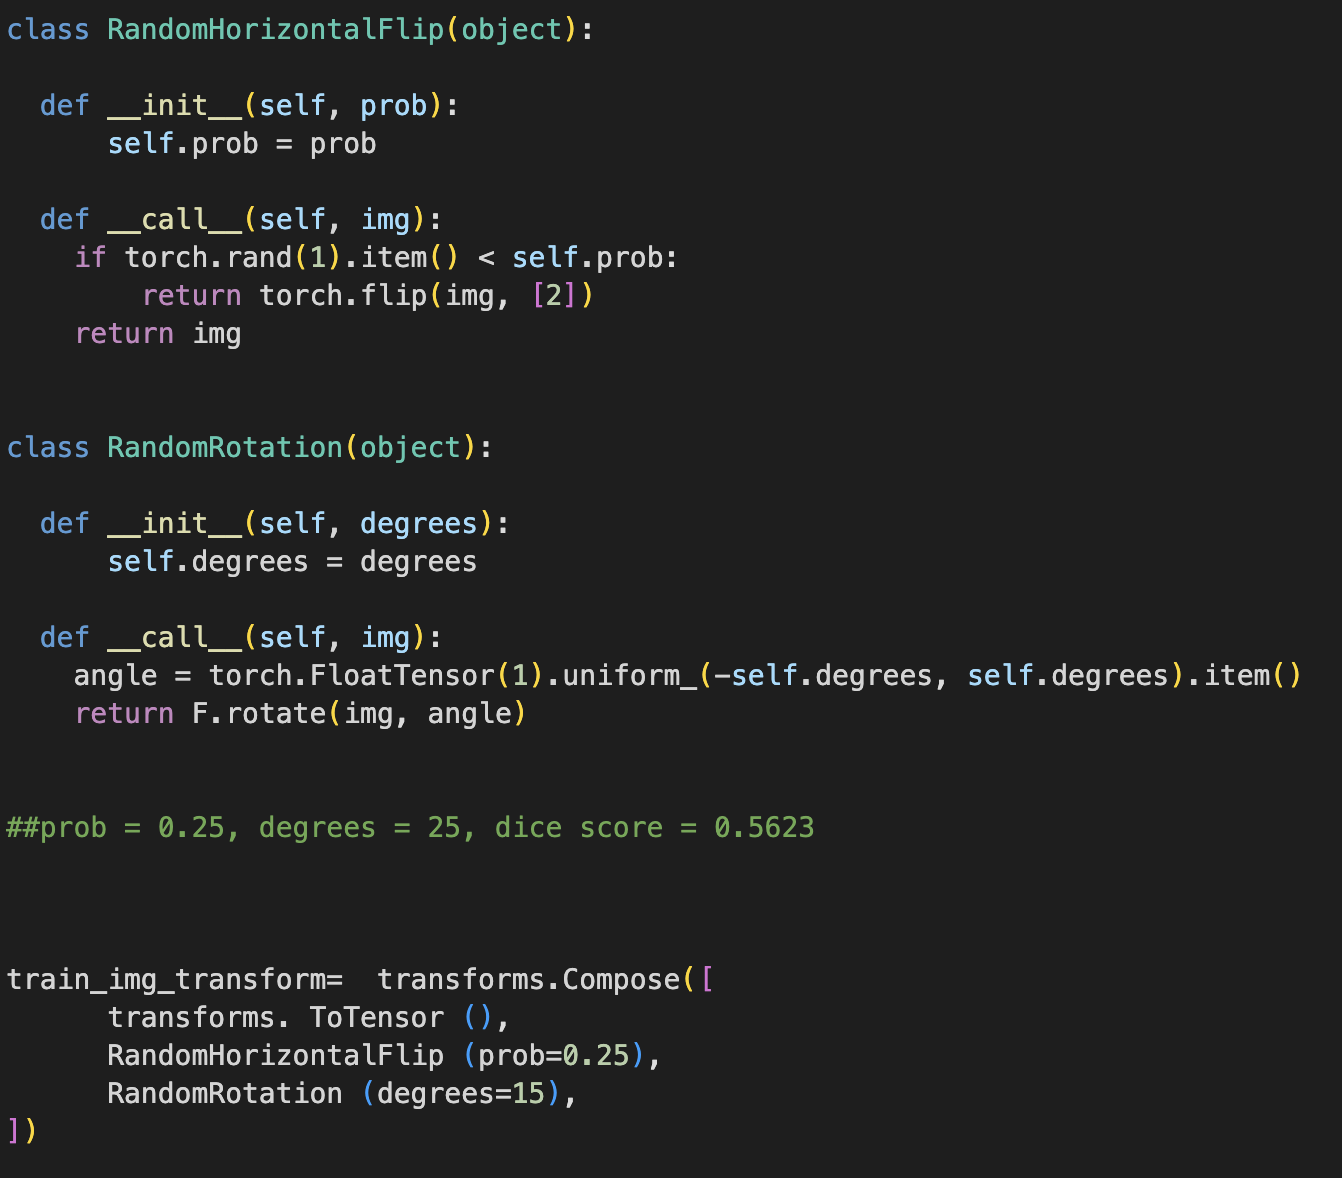
\includegraphics[width= 0.8\textwidth]{/Users/zhangxiangyu/JHU/Fall 2023/deep learning/hw6/fig/1b_aug.png}
				\caption{Data augmentation}
				\label{fig:1b_aug}
			\end{figure}

			\begin{figure}[H]
				\centering
				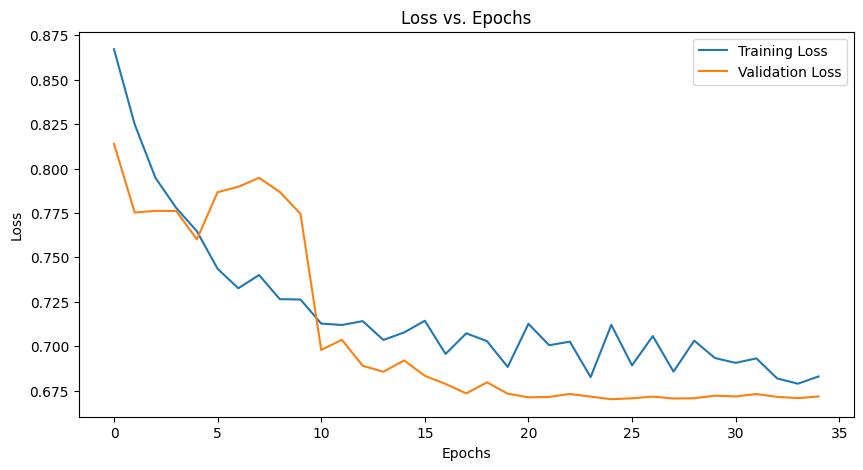
\includegraphics[width= 1.0\textwidth]{/Users/zhangxiangyu/JHU/Fall 2023/deep learning/hw6/fig/1b.png}
				\caption{Validation and train loss w.r.t. epochs}
				\label{fig:1b}
			\end{figure}

			\begin{figure}[H]
				\centering
				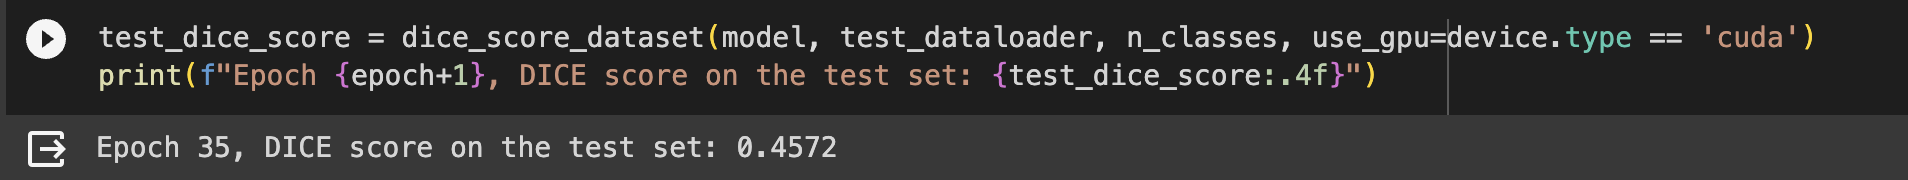
\includegraphics[width= 0.9\textwidth]{/Users/zhangxiangyu/JHU/Fall 2023/deep learning/hw6/fig/1b_dice.png}
				\caption{Dice score on the test dataset}
				\label{fig:1b_dice}
			\end{figure}


			
			


			\item Train on the colorization task using frames from the `/colorization/train\_cor' folder. Use hyperparameters that seem reasonable (based on your previous experiments) and mean squared error as your loss function. Please provide a figure of training loss w.r.t. epochs until your model converges. Then save your model to initialize the network for the next task.
			
			\noindent \textbf{Answer for 1(c):} \\

			The training loss of colorization task can be found in Figure ~\ref{fig:1c}. 

			\begin{figure}[H]
				\centering
				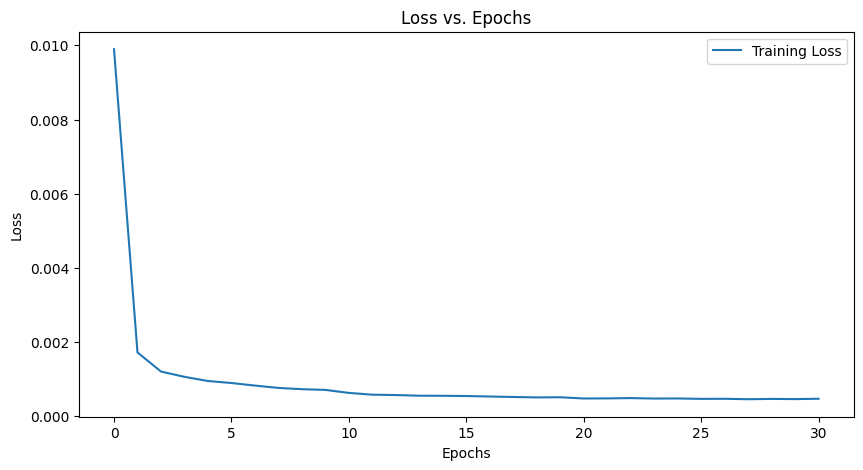
\includegraphics[width= 0.9\textwidth]{/Users/zhangxiangyu/JHU/Fall 2023/deep learning/hw6/fig/loss.png}
				\caption{Training loss of colorization task}
				\label{fig:1c}
			\end{figure}

			And the recolorized images can be found in Figure ~\ref{fig:1c_color}.

			\begin{figure}[H]
				\centering
				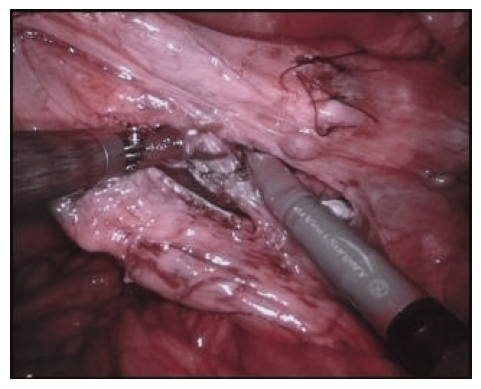
\includegraphics[width= 0.8\textwidth]{/Users/zhangxiangyu/JHU/Fall 2023/deep learning/hw6/fig/recolorization.png}
				\caption{Recolorized images}
				\label{fig:1c_color}
			\end{figure}


			\item Load the colorization pre-trained model and start training for the segmentation task using the frames in the `/segmentation/train' folder. Make sure you are using the same hyperparameters as you did in the former task, and please clearly state  them in your report. Plot the figure of training loss and validation loss. Report test dataset performance. Do you see a difference with the former result in (b)? (\textit{Hint: Since this is a relatively simple dataset, you might not actually observe differences in performance.})  
			
			\noindent \textbf{Answer for 1(d):} \\	

			The training loss and validation loss can be found in Figure ~\ref{fig:1d}. The dice score on the test dataset is $0.4896$, which can be shown in Figure ~\ref{fig:1d_dice}.

			There is not much difference between the result in (b) and (d). The possible reason is our small data set may not have enough variation to train a model to recognize complex patterns in new samples.
			\begin{figure}[H]
				\centering
				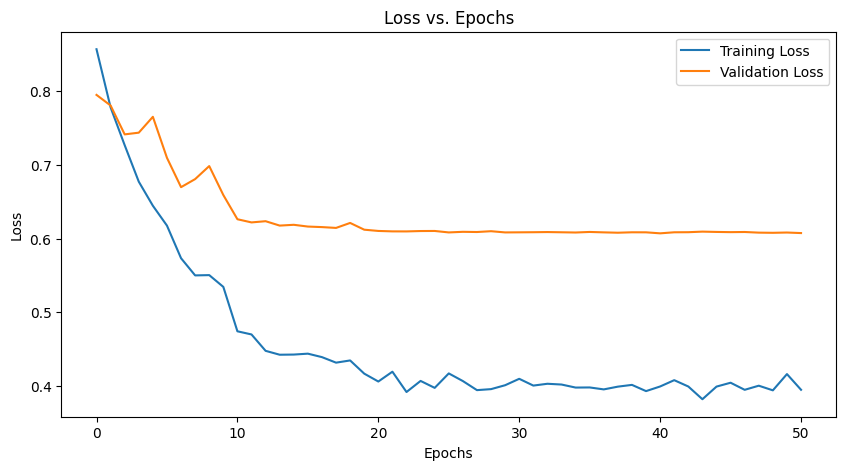
\includegraphics[width= 1.0\textwidth]{/Users/zhangxiangyu/JHU/Fall 2023/deep learning/hw6/fig/1d.png}
				\caption{Validation and train loss w.r.t. epochs}
				\label{fig:1d}
			\end{figure}

			\begin{figure}[H]
				\centering
				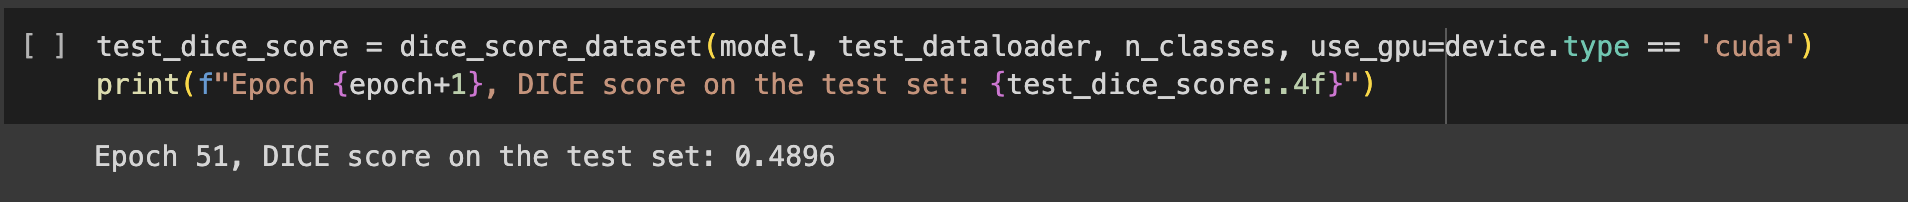
\includegraphics[width= 0.9\textwidth]{/Users/zhangxiangyu/JHU/Fall 2023/deep learning/hw6/fig/Screenshot 2023-11-09 at 2.41.54 AM.png}
				\caption{Dice score on the test dataset}
				\label{fig:1d_dice}
			\end{figure}



		\end{enumerate}
	
		
		% Problem 2
		\item \textit{Transfer Learning}. Please download the fashion MNIST dataset \footnote{The full FashionMNIST dataset can be downloaded from the official website here: \url{https://github.com/zalandoresearch/fashion-mnist}} as used in HW4 and download the VGG16 model (\url{https://pytorch.org/docs/stable/torchvision/models.html}). 
		\begin{enumerate}
			\item Randomly initialize all parameters in VGG16 and try to train your model to learn the Fashion MNIST classification task. What's the accuracy you achieve? Please report your test accuracy on the test dataset. You should expect an accuracy > 85\%.
			
			\noindent \textbf{Answer for 2(a):} \\
			The accuracy on train dataset is 0.9204 and the test accuracy is 0.9156.
			\begin{figure}[H]
				\centering
				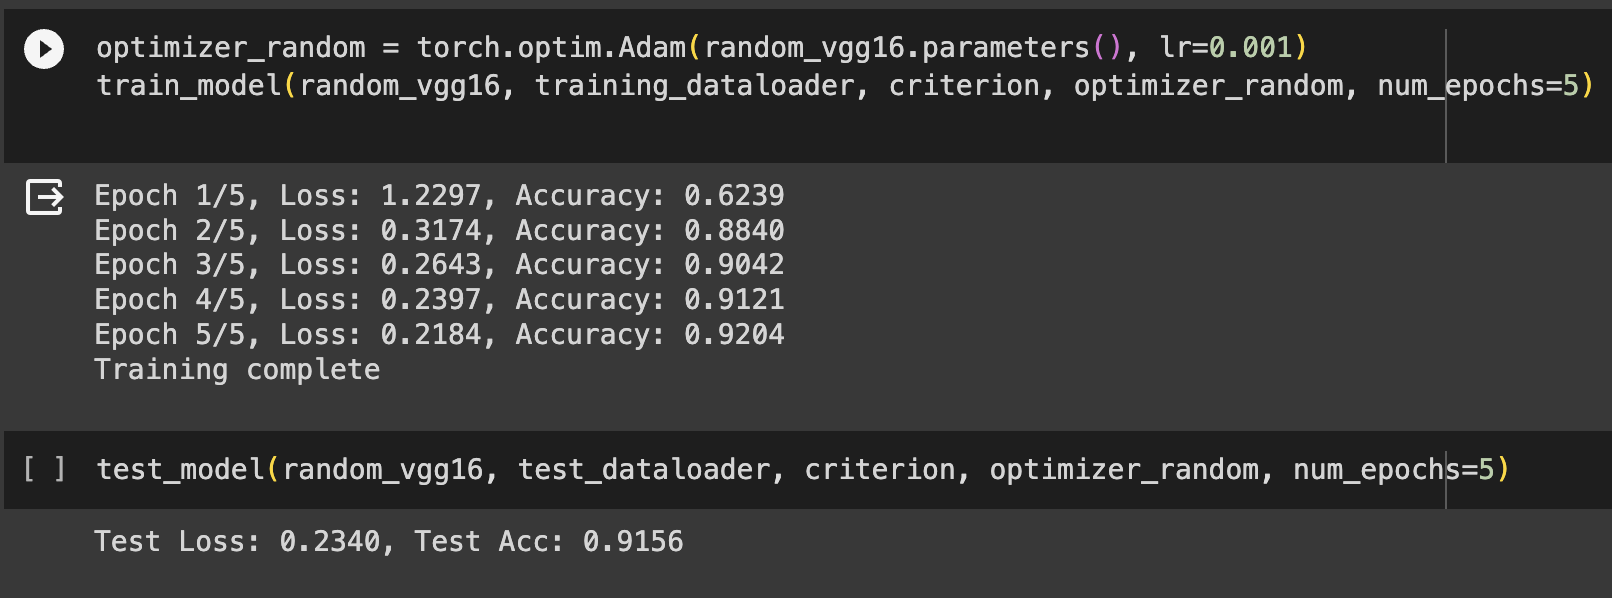
\includegraphics[width= 0.9\textwidth]{/Users/zhangxiangyu/JHU/Fall 2023/deep learning/hw6/fig/Screenshot 2023-11-09 at 2.47.09 AM.png}
				\caption{Train acc and Test acc}
				\label{fig:1d_dice}
			\end{figure}



			\item Load the pre-trained VGG16 model from torch vision models. Freeze all but the last layer: randomly initialize the last layer of your network and fine-tune this. What accuracy do you get now? Please again report your test accuracy on the test dataset. You should expect an accuracy > 60\%.
			
			\noindent \textbf{Answer for 2(b):} \\
			The accuracy on train dataset is 0.8191 and the test accuracy is 0.8498.
			\begin{figure}[H]
				\centering
				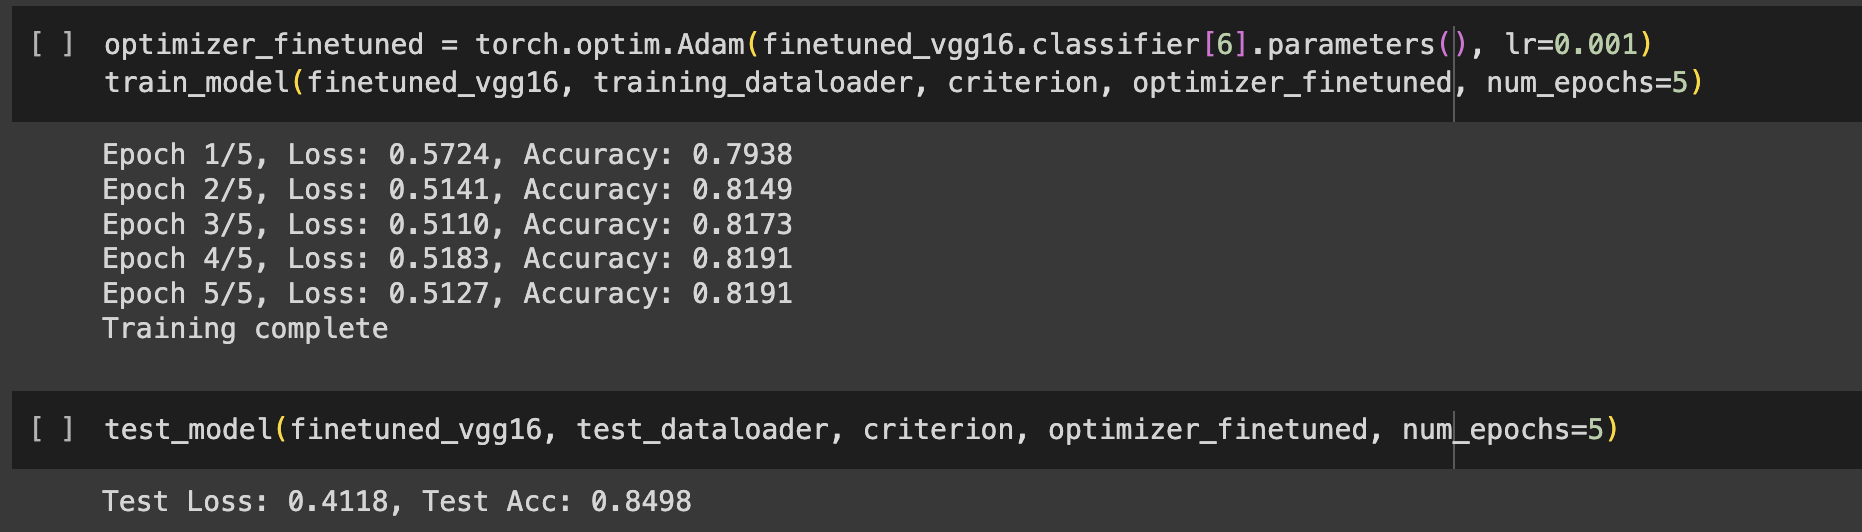
\includegraphics[width= 0.9\textwidth]{/Users/zhangxiangyu/JHU/Fall 2023/deep learning/hw6/fig/Screenshot 2023-11-09 at 2.49.42 AM.png}
				\caption{Train acc and Test acc}
				\label{fig:1d_dice}
			\end{figure}



			\item Now, imagine a scenario in which you want to train the VGG16 model on an entirely new dataset and will fine-tune either the model from (2a) or (2b). Which pre-trained model is the preferred starting point for your new use case?
			
			\noindent \textbf{Answer for 2(c):} \\

			Starting with the pre-trained VGG16 model (as described in scenario 2b) maybe a better choice. Since the model has already learned a variety of features from a large and diverse dataset. This knowledge provides a useful starting point for learning new tasks, even if the new dataset is quite different from the original training data. \\
			Also, 2b model provides better feature extraction capabilities and generalization performance
		\end{enumerate} 
	\end{enumerate}
\end{document}















